\section{Descripción de los Datos} \label{descr-datos}

\subsection{Descripción preliminar de los datos}

Se cuenta con un \textit{dataset}, obtenido de \href{https://www.kaggle.com/rtatman/188-million-us-wildfires}{Kaggle}, con un registro de 1.880.465 incendios históricos ocurridos en Estados Unidos, desde 1992 hasta 2015. La información original se obtuvo a partir del \textit{U.S. Department of Agriculture} \cite{FPA}.

El \textit{dataset} se encuentra en extensión \textit{.sqlite}, de donde ocuparemos la tabla ``\textit{Fires}'', que posee en total 37 columnas, dentro de las cuales, existen columnas para describir el ID (como lo es \textit{\textbf{FOD\_ID}} O \textit{\textbf{FPA\_ID}}), las siglas (como lo es \textit{\textbf{STATE}}), los nombres (como lo es \textit{\textbf{SOURCE\_SYSTEM\_TYPE}}), algunos parámetros numéricos (como lo es \textit{\textbf{FIRE\_SIZE}}), parámetros temporales (como lo es \textit{\textbf{CONT\_DATE}} o \textit{\textbf{CONT\_TIME}}), parámetros espaciales (como lo es \textit{\textbf{LATITUDE}}), entre otros (que no viene al caso describir cada una de las columnas del \textit{dataset}, dado a que posee una cantidad abrumadora de columnas). Dentro de las cuales, la columna de etiquetas (que en nuestro caso viene a ser lo mismo que las causas) que se desea predecir es la llamada \textit{\textbf{STAT\_CAUSE\_DESCR}}.

Para más información acerca de las columnas del \textit{dataset}, se puede consultar la documentación proporcionada en la página de Kaggle.

\subsection{Descripción de las columnas a ocupar}

Del total de columnas que posee la tabla, ocuparemos aquellas que estén relacionadas con la fecha (como la hora y la fecha estimada en que se inició el incendio y el momento en que se controló), la geografía (como las siglas del estado en que se originó el incendio, y la latitud y longitud del incendio), el tamaño del incendio y la descripción de la causa del incendio (que es la variable objetivo a predecir). 

El resto de variables no representan información relevante para predecir las causas de un incendio. Por ejemplo, el ID del incendio, o del departamento que logró controlar el incendió, no aporta información importante a la causa del incendio, pues no es una propiedad ``\textit{natural}'' del mismo (es más, puede resultar en un sesgo a la hora de predecir).

A continuación se describirán brevemente las columnas que se ocuparán:
\begin{enumerate}
    \item \textit{\textbf{FIRE\_YEAR}}: Corresponde al año en que se originó el incendio. Es una variable temporal.
    \item \textit{\textbf{DISCOVERY\_DATE}}: Es la fecha (estimada) en que se originó el incendio. Es una variable temporal que, inicialmente, es del tipo float.
    \item \textit{\textbf{DISCOVERY\_TIME}}: Es la hora (estimada) en que se originó el incendio. Es una variable temporal que, inicialmente, es de tipo cadena.
    \item \textit{\textbf{STAT\_CAUSE\_DESCR}}: Es la causa que originó el incendio. Es una variable categórica de tipo cadena
    \item \textit{\textbf{CONT\_DATE}}: Es la fecha en que se logró extinguir el incendio. Es una variable temporal que, inicialmente, es del tipo float.
    \item \textit{\textbf{CONT\_TIME}}: Es la hora en que se logró extinguir el incendio. Es una variable temporal que, inicialmente, es de tipo cadena.
    \item \textit{\textbf{FIRE\_SIZE}}: Es la extensión (área) que tuvo el incendio (medido en Acres). Es una variable numérica.
    \item \textit{\textbf{FIRE\_SIZE\_CLASS}}: Es una clasificación que utilizan los bomberos para describir la extensión del incendio. Es una variable categórica.
    \item \textit{\textbf{LATITUDE}}: Es la latitud del incendio. Es una variable numérica.
    \item \textit{\textbf{LONGITUDE}}: Es la longitud del incendio. Es una variable numérica.
    \item \textit{\textbf{STATE}}: Es el estado en que se originó el incendio. Es una variable categórica.
\end{enumerate}

\subsection{Descripción del dataset con las columnas a ocupar} \label{descr-dataset}

Restringido a las columnas mencionadas anteriormente, se observa que el \textit{dataset} posee un total de 3.535 filas duplicadas. 

También se observa que las siguientes columnas poseen valores nulos: 
\begin{itemize}
    \item \ColStyle{DISCOVERY\_TIME}, con un total de 882.638 valores nulos,
    \item \ColStyle{CONT\_DATE}, con un total de 891.531 valores nulos, y
    \item \ColStyle{CONT\_TIME}, con un total de 972.173 valores nulos.
\end{itemize}

Además, se observa que las columnas relacionadas con las fechas se encuentran en un formato de fecha juliana\footnote{Esto corresponde al número de días transcurridos desde el mediodía del 1° de enero del año 4713 a. C.} y que las columnas relacionadas a las horas son cadenas, se encuentran en formato ``HHMM'', donde HH corresponde al número de horas y MM corresponde al número de minutos.

Finalmente, cabe mencionar que la columna \ColStyle{FIRE\_SIZE} corresponde al área total en que se propagó el incendio, medido en Acres\footnote{Un acre corresponde a 4046.85 metros cuadrados.}.

\subsection{Descripción de las etiquetas de la columna objetivo}

A continuación, describiremos brevemente las etiquetas que posee la columna que se desea predecir, \textit{\textbf{STAT\_CAUSE\_DESCR}}:
\begin{itemize}
    \item \textbf{Miscellaneous}: de causa Miscelánea.
    \item \textbf{Children}: Causado por infantes.
    \item \textbf{Lightning}: Causado por un rayo.
    \item \textbf{Smoking}: Causado por un cigarrillo mal apagado.
    \item \textbf{Arson}: Causado con fines maliciosos.
    \item \textbf{Equipment Use}: Causado por el uso de un equipamiento.
    \item \textbf{Debris Burning}: Causado por quema de escombros.
    \item \textbf{Campfire}: Causado por un campamento.
    \item \textbf{Railroad}: Causado por un ferrocarril.
    \item \textbf{Missing/Undefined}: Que tiene datos faltantes o que no están definidos.
    \item \textbf{Powerline}: Causado por la linea eléctrica.
    \item \textbf{Fireworks}: Causado por fuegos artificiales.
    \item \textbf{Structure}: Causado por Estructura.
\end{itemize}

Cabe destacar, que en la documentación de la base de datos no aparece una descripción detallada de las categorías. Con lo que, varias de las descripciones de estas causas fueron inferidas por el autor.

\section{Tratamiento de los Datos}
\subsection{Limpieza preliminar de los datos}
Como se comentó en la sección \ref{descr-dataset}, el \textit{dataset} posee algunos datos duplicados o con valores nulos. Para remediar esto, se procede a eliminar estas filas, resultando en un \textit{dataset} de 890.821 filas, aproximadamente la mitad de datos que poseía el \textit{dataset} originalmente.

\subsection{Tratamiento de las columnas de fecha y hora}
Como se comentó en la sección \ref{descr-dataset}, las fechas se encuentran en formato de fecha juliana, y el tiempo se encuentra en formato ``HHMM''.

Para tratar con estos formatos, primero se transforma las fechas en formato gregoriano\footnote{Es decir, en un formato AAAA-MM-DD, donde AAAA es el año, MM es el mes y DD es el día.}, y las horas se transforman en un formato más estándar, digamos, ``HH:MM:SS'', con SS los segundos (donde como no se posee la información de los segundos, se rellenan con 00). Paso seguido, se utiliza la fecha y la hora para transforlas en datos del tipo \textit{DateTime}. Esto se realiza para las columnas de sufijo \textit{\textbf{DISCOVERY\_*}} y \textit{\textbf{CONT\_*}}. De esta forma, 4 de las columnas que se tenían anteriormente, se resumen en dos columnas, las cuales se nombraron \ColStyle{DISC\_DATE\_TIME} y \ColStyle{CONT\_DATE\_TIME}.

\subsection{Creación de nuevas columnas}

A partir de las nuevas columnas creadas, \ColStyle{$\{$DISC,CONT$\}$\_DATE\_TIME}, se crean las siguientes columnas:
\begin{itemize}
    \item \ColStyle{$\{$DISC,CONT$\}$\_MONTH}: Columna que indica el mes de descubrimiento/contención del incendio.
    \item \ColStyle{$\{$DISC,CONT$\}$\_DAY\_OF\_WEEK}: Columna que indica el día de la semana del descubrimiento/contención del incendio.
    \item \ColStyle{DT\_FIRE}: Columna que indica el número de horas utilizadas en controlar el incendio.
\end{itemize}

\subsection{Ordenación del dataset con respecto a la fecha}\label{ord-cr-fecha}
Por razones que se explicarán más adelante (específicamente en la sección \ref{prep-train-test}), el \textit{dataset} se organiza con respecto a la columna \ColStyle{DISC\_DATE\_TIME}, es decir, se organiza con respecto a la fecha y a la hora.

\subsection{Creación de nuevas categorías}\label{subsec:nuevas-cats}
Más adelante se observará que existen categorías bastante mayoritarias frente a otras. Para solucionar este problema, se propondrá una recategorización, que consiste en hacer 4 nuevas categorías:
\begin{itemize}
    \item \textbf{Natural}: Causas naturales. \textit{Lightning} entra en esta categoría.
    \item \textbf{Malicious}: Causas maliciosas. \textit{Arson} entra en esta categoría.
    \item \textbf{Other}: Causas que no se especifican bien. \textbf{Miscellaneous} y \textbf{Missing/Undefined} entran en esta categoría
    \item \textbf{Human}: Hecha por causas humanas, y que probablemente fueron accidente. El resto de las causas que no han sido mencionadas entran en esta categoría.
\end{itemize}

\begin{figure}[!t]
    \centering
    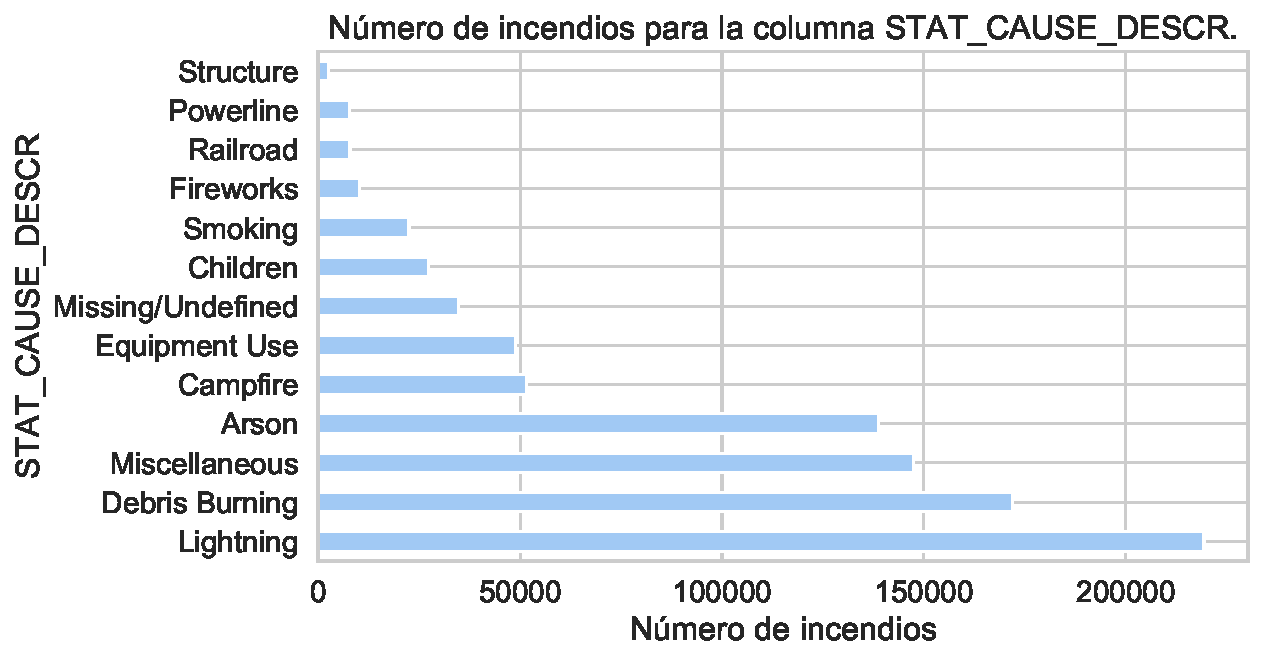
\includegraphics[width=0.48\textwidth]{imagenes/barh_STAT_CAUSE_DESCR.pdf}
    \caption{Gráfico de Causas vs. Número de incendios.}
    \label{fig:SCD}
\end{figure}
\section{Análisis Exploratorio de los Datos}\label{EDA}
La primera pregunta que alguien se puede realizar es: ¿Cómo están distribuidos el número de incendios con respecto a la causa del incendio? Para responder a la interrogante, se procede a graficar el número de incendios con respecto a sus causas. El resultado del gráfico se puede observar en la Fig.~\ref{fig:SCD}.

Se puede observar que las principales causas de incendio son producidos por rayos (\textit{Lightning}), quema de escombros (\textit{Debris Burning}), de forma miscelánea (\textit{Miscellaneous}) y por razones maliciosas (\textit{Arson}). Mientras que el resto de causas tienen un papel minoritario. 

También, otra de las primeras observaciones que se pueden rescatar, es que el \textit{dataset} se encuentra \textit{desequilibrado} (i.e., que existen clases bastante más númerosas que otras). Esto causará que a la hora de realizar clasificación, las clases con mayor número de incendios (como \textit{Lightning}) queden beneficiadas frente a las clases minoritarias (como \textit{Structure}), resultando en \textit{overfitting}.

Para solucionar este problema, se crearán 4 nuevas categorías, como se explica en \ref{subsec:nuevas-cats}. estas son: \textbf{Natural}, \textbf{Malicious}, \textbf{Other} y \textbf{Human}. En la Fig.~\ref{fig:SCDN} se puede observar la nueva distribución que resulta de la creación de las nuevas categorías.
\begin{figure}
    \centering
    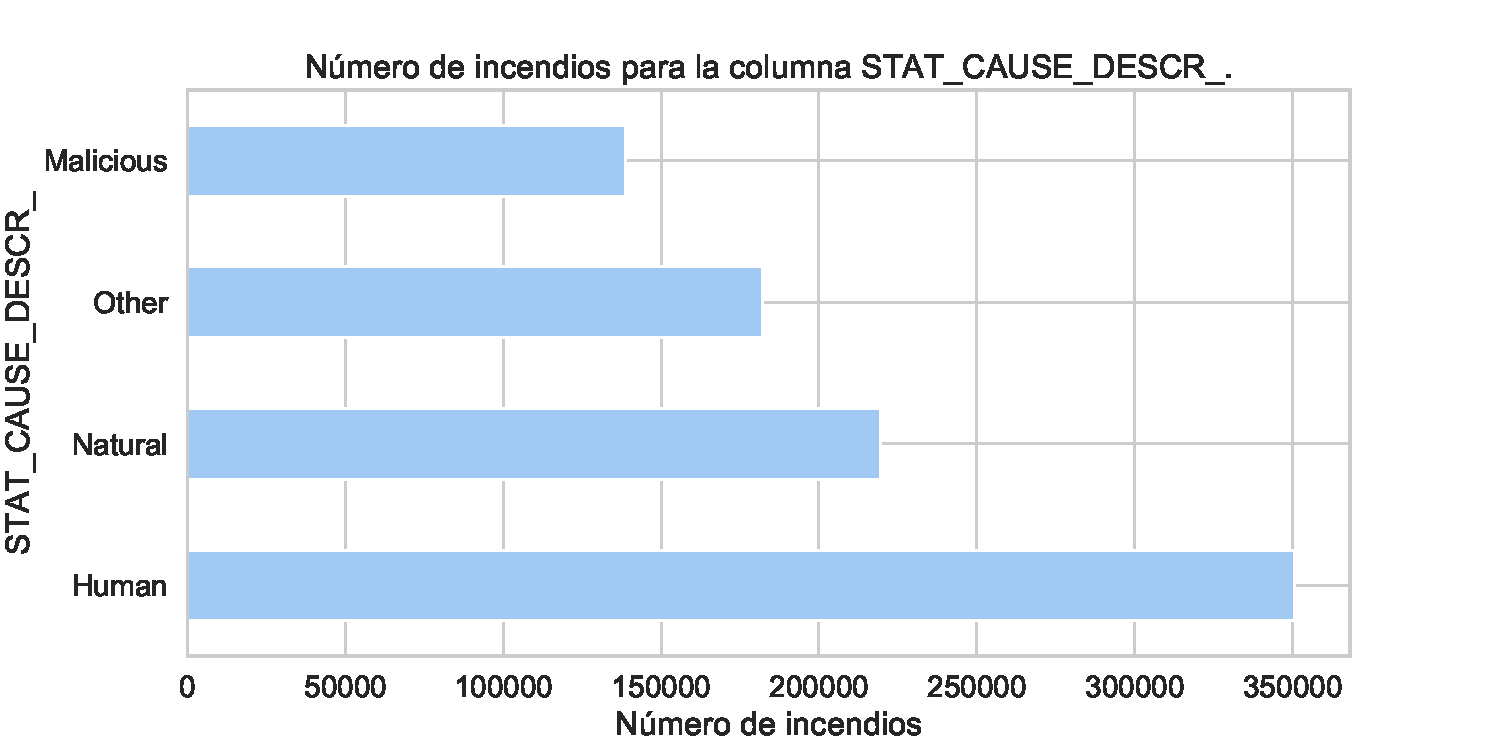
\includegraphics[width=0.48\textwidth]{imagenes/barh_STAT_CAUSE_DESCR_.pdf}
    \caption{Gráfico de Causas Nuevas vs. Número de incendios.}
    \label{fig:SCDN}
\end{figure}

Se puede observar a primera vista que la nueva categorización resulta en un \textit{dataset} más balanceado, y que además, la causa humana resulta ser la nueva clase mayoritaria.

Otra interrogante que se puede plantear es: ¿Cómo se distribuyen los incendios a lo largo de los años? Para responder a esta pregunta, se elaboró un gráfico del número de incendios vs. el año de ocurrencia. El resultado del gráfico se puede observar en la Fig.~\ref{fig:Year-Ocurr}.
\begin{figure}
    \centering
    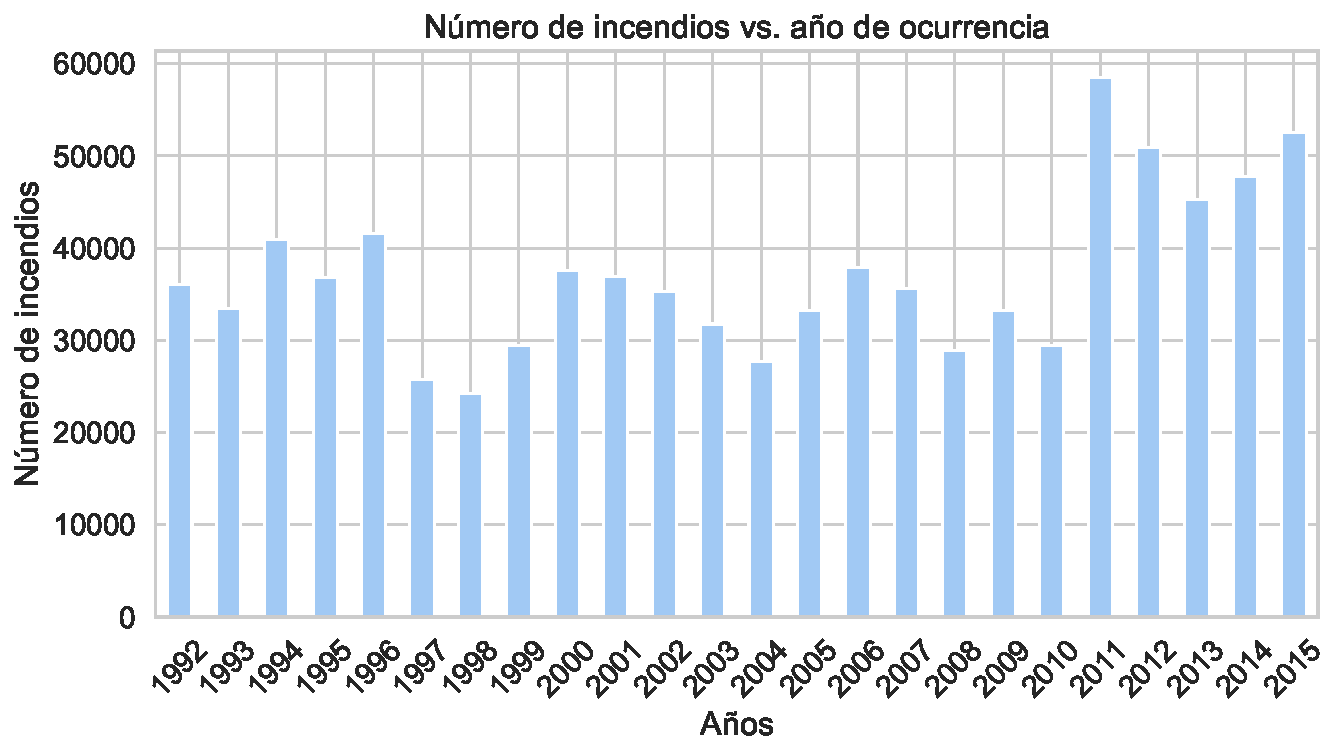
\includegraphics[width=0.48\textwidth]{imagenes/YEAR_OCURRENCIA.pdf}
    \caption{Gráfico de Número de incendios vs. Año de ocurrencia.}
    \label{fig:Year-Ocurr}
\end{figure}

Las primeras apreciaciones que se observan es que en los últimos años (desde el 2011 hasta el 2015) se tuvo un alza importante de incendios. Quizás, esto se puede deber a que en los últimos años se cambió la forma en que se contabilizaban los incendios, o quizás que en esos años ocurrieron incendios con el interés de ocupar el terreno.

Además, también se observa que hay años que son minoría comparativamente, como por ejemplo, en el año 2011 ocurrieron más del doble de incendios que en el año 1998. 

Es importante tomar en cuenta estas observaciones, pues puede afectar en la predicción del clasificador en gran medida, pues este no estará consciente de las ``rachas'' de incendios que ocurrieron en los últimos años.












% Visualizaciones y resultados relevantes.

% - Análisis exploratorio de datos, mostrar solo visualizaciones y resultados relevantes.
% - Lo realizado para la presentación 1 (que en algunos casos sería lo mismo del análisis exploratorio, o los primeros problemas que tuvieron con sus bases de datos o problemas)
% - Lo realizado para la presentación 2, que sería mostrar en algunos casos el primer experimento que realizaron para resolver su problema, o en otros sería plantear el por qué cambiaron su problema o base de datos.